\documentclass[12pt,a4paper]{report}
\usepackage[T1]{fontenc}
\usepackage[utf8]{inputenc}
\usepackage{mathptmx}
\usepackage[margin=25mm]{geometry}
\usepackage{graphicx,xcolor,pdflscape,fancyhdr,hyperref}
\definecolor{epsblue}{HTML}{1764A0}
\hypersetup{colorlinks=true,linkcolor=epsblue,urlcolor=epsblue,pdftitle={EPS Sequence Diagrams}}
\setlength{\headheight}{15pt}
\setlength{\parskip}{4pt}
\pagestyle{fancy}\fancyhf{}
\fancyhead[L]{Systems Analysis and Design - IT3120E}
\fancyhead[R]{EPS Sequence Diagrams}
\fancyfoot[C]{\thepage}
\newcommand{\epsfigure}[3]{\clearpage\begin{figure}[p]\centering\includegraphics[width=\textwidth,height=0.87\textheight,keepaspectratio,clip]{#1}\caption{#2}\label{#3}\end{figure}\clearpage}
\newlength{\epsavailable}\newcommand{\epsfirstfigure}[3]{\par\setlength{\epsavailable}{\dimexpr\textheight-\pagetotal-70pt\relax}\ifdim\epsavailable<0.48\textheight\clearpage\setlength{\epsavailable}{0.87\textheight}\fi\ifdim\epsavailable>0.87\textheight\setlength{\epsavailable}{0.87\textheight}\fi\begin{figure}[!ht]\centering\includegraphics[width=\textwidth,height=\epsavailable,keepaspectratio,clip]{#1}\caption{#2}\label{#3}\end{figure}\clearpage}
\begin{document}
\setcounter{chapter}{3}\setcounter{section}{3}
\setcounter{figure}{28}
\section{Sequence Diagram}
Sequence diagrams show actor, boundary, control and entity interactions. Large flows continue in the referenced modules; B1.API and U4.API use the same business rules as their user-interface variants.

\subsection{User's Use cases}
\epsfirstfigure{diagrams/sequence/SD_U1.pdf}{U1: Register}{fig:sequence-u1}
\epsfigure{diagrams/sequence/SD_U1_enrollment.pdf}{U1: Register (continued: U1\_\allowbreak{}enrollment)}{fig:sequence-u1-enrollment}
\epsfigure{diagrams/sequence/SD_U2.pdf}{U2: Login with MFA}{fig:sequence-u2}
\epsfigure{diagrams/sequence/SD_U2_mfa.pdf}{U2: Login with MFA (continued: U2\_\allowbreak{}mfa)}{fig:sequence-u2-mfa}
\epsfigure{diagrams/sequence/SD_U3.pdf}{U3: Logout}{fig:sequence-u3}
\epsfigure{diagrams/sequence/SD_U3_authorized_flow.pdf}{U3: Logout (continued: U3\_\allowbreak{}authorized\_\allowbreak{}flow)}{fig:sequence-u3-authorized-flow}
\epsfigure{diagrams/sequence/SD_U4.pdf}{U4: View/Track Escrows}{fig:sequence-u4}
\epsfigure{diagrams/sequence/SD_U4_outcomes.pdf}{U4: View/Track Escrows (continued: U4\_\allowbreak{}outcomes)}{fig:sequence-u4-outcomes}
\epsfigure{diagrams/sequence/SD_U4_tracking.pdf}{U4: View/Track Escrows (continued: U4\_\allowbreak{}tracking)}{fig:sequence-u4-tracking}
\epsfigure{diagrams/sequence/SD_U4.API.pdf}{U4.API: View/Track Escrows}{fig:sequence-u4-api}
\epsfigure{diagrams/sequence/SD_U4.API_authorized_request.pdf}{U4.API: View/Track Escrows (continued: U4.API\_\allowbreak{}authorized\_\allowbreak{}request)}{fig:sequence-u4-api-authorized-request}
\epsfigure{diagrams/sequence/SD_U4.API_outcomes.pdf}{U4.API: View/Track Escrows (continued: U4.API\_\allowbreak{}outcomes)}{fig:sequence-u4-api-outcomes}
\epsfigure{diagrams/sequence/SD_U5.pdf}{U5: Open Dispute}{fig:sequence-u5}
\epsfigure{diagrams/sequence/SD_U5_outcomes.pdf}{U5: Open Dispute (continued: U5\_\allowbreak{}outcomes)}{fig:sequence-u5-outcomes}
\epsfigure{diagrams/sequence/SD_U6.pdf}{U6: Submit Dispute Evidence}{fig:sequence-u6}
\epsfigure{diagrams/sequence/SD_U6_outcomes.pdf}{U6: Submit Dispute Evidence (continued: U6\_\allowbreak{}outcomes)}{fig:sequence-u6-outcomes}
\epsfigure{diagrams/sequence/SD_U7.pdf}{U7: Propose/Withdraw Full Refund}{fig:sequence-u7}
\epsfigure{diagrams/sequence/SD_U7_outcomes.pdf}{U7: Propose/Withdraw Full Refund (continued: U7\_\allowbreak{}outcomes)}{fig:sequence-u7-outcomes}
\epsfigure{diagrams/sequence/SD_U8.pdf}{U8: Accept/Reject Refund Proposal}{fig:sequence-u8}
\epsfigure{diagrams/sequence/SD_U8_outcomes.pdf}{U8: Accept/Reject Refund Proposal (continued: U8\_\allowbreak{}outcomes)}{fig:sequence-u8-outcomes}
\epsfigure{diagrams/sequence/SD_U8_accept_refund.pdf}{U8: Accept/Reject Refund Proposal (continued: U8\_\allowbreak{}accept\_\allowbreak{}refund)}{fig:sequence-u8-accept-refund}
\subsection{Buyer's Use cases}
\epsfirstfigure{diagrams/sequence/SD_B1.pdf}{B1: Create Escrow}{fig:sequence-b1}
\epsfigure{diagrams/sequence/SD_B1_outcomes.pdf}{B1: Create Escrow (continued: B1\_\allowbreak{}outcomes)}{fig:sequence-b1-outcomes}
\epsfigure{diagrams/sequence/SD_B1.API.pdf}{B1.API: Create Escrow}{fig:sequence-b1-api}
\epsfigure{diagrams/sequence/SD_B1.API_authorized_request.pdf}{B1.API: Create Escrow (continued: B1.API\_\allowbreak{}authorized\_\allowbreak{}request)}{fig:sequence-b1-api-authorized-request}
\epsfigure{diagrams/sequence/SD_B2.pdf}{B2: Cancel Unfunded Escrow}{fig:sequence-b2}
\epsfigure{diagrams/sequence/SD_B2_outcomes.pdf}{B2: Cancel Unfunded Escrow (continued: B2\_\allowbreak{}outcomes)}{fig:sequence-b2-outcomes}
\clearpage\newgeometry{margin=15mm,headheight=15pt,headsep=8pt,footskip=16pt}\begin{figure}[p]\centering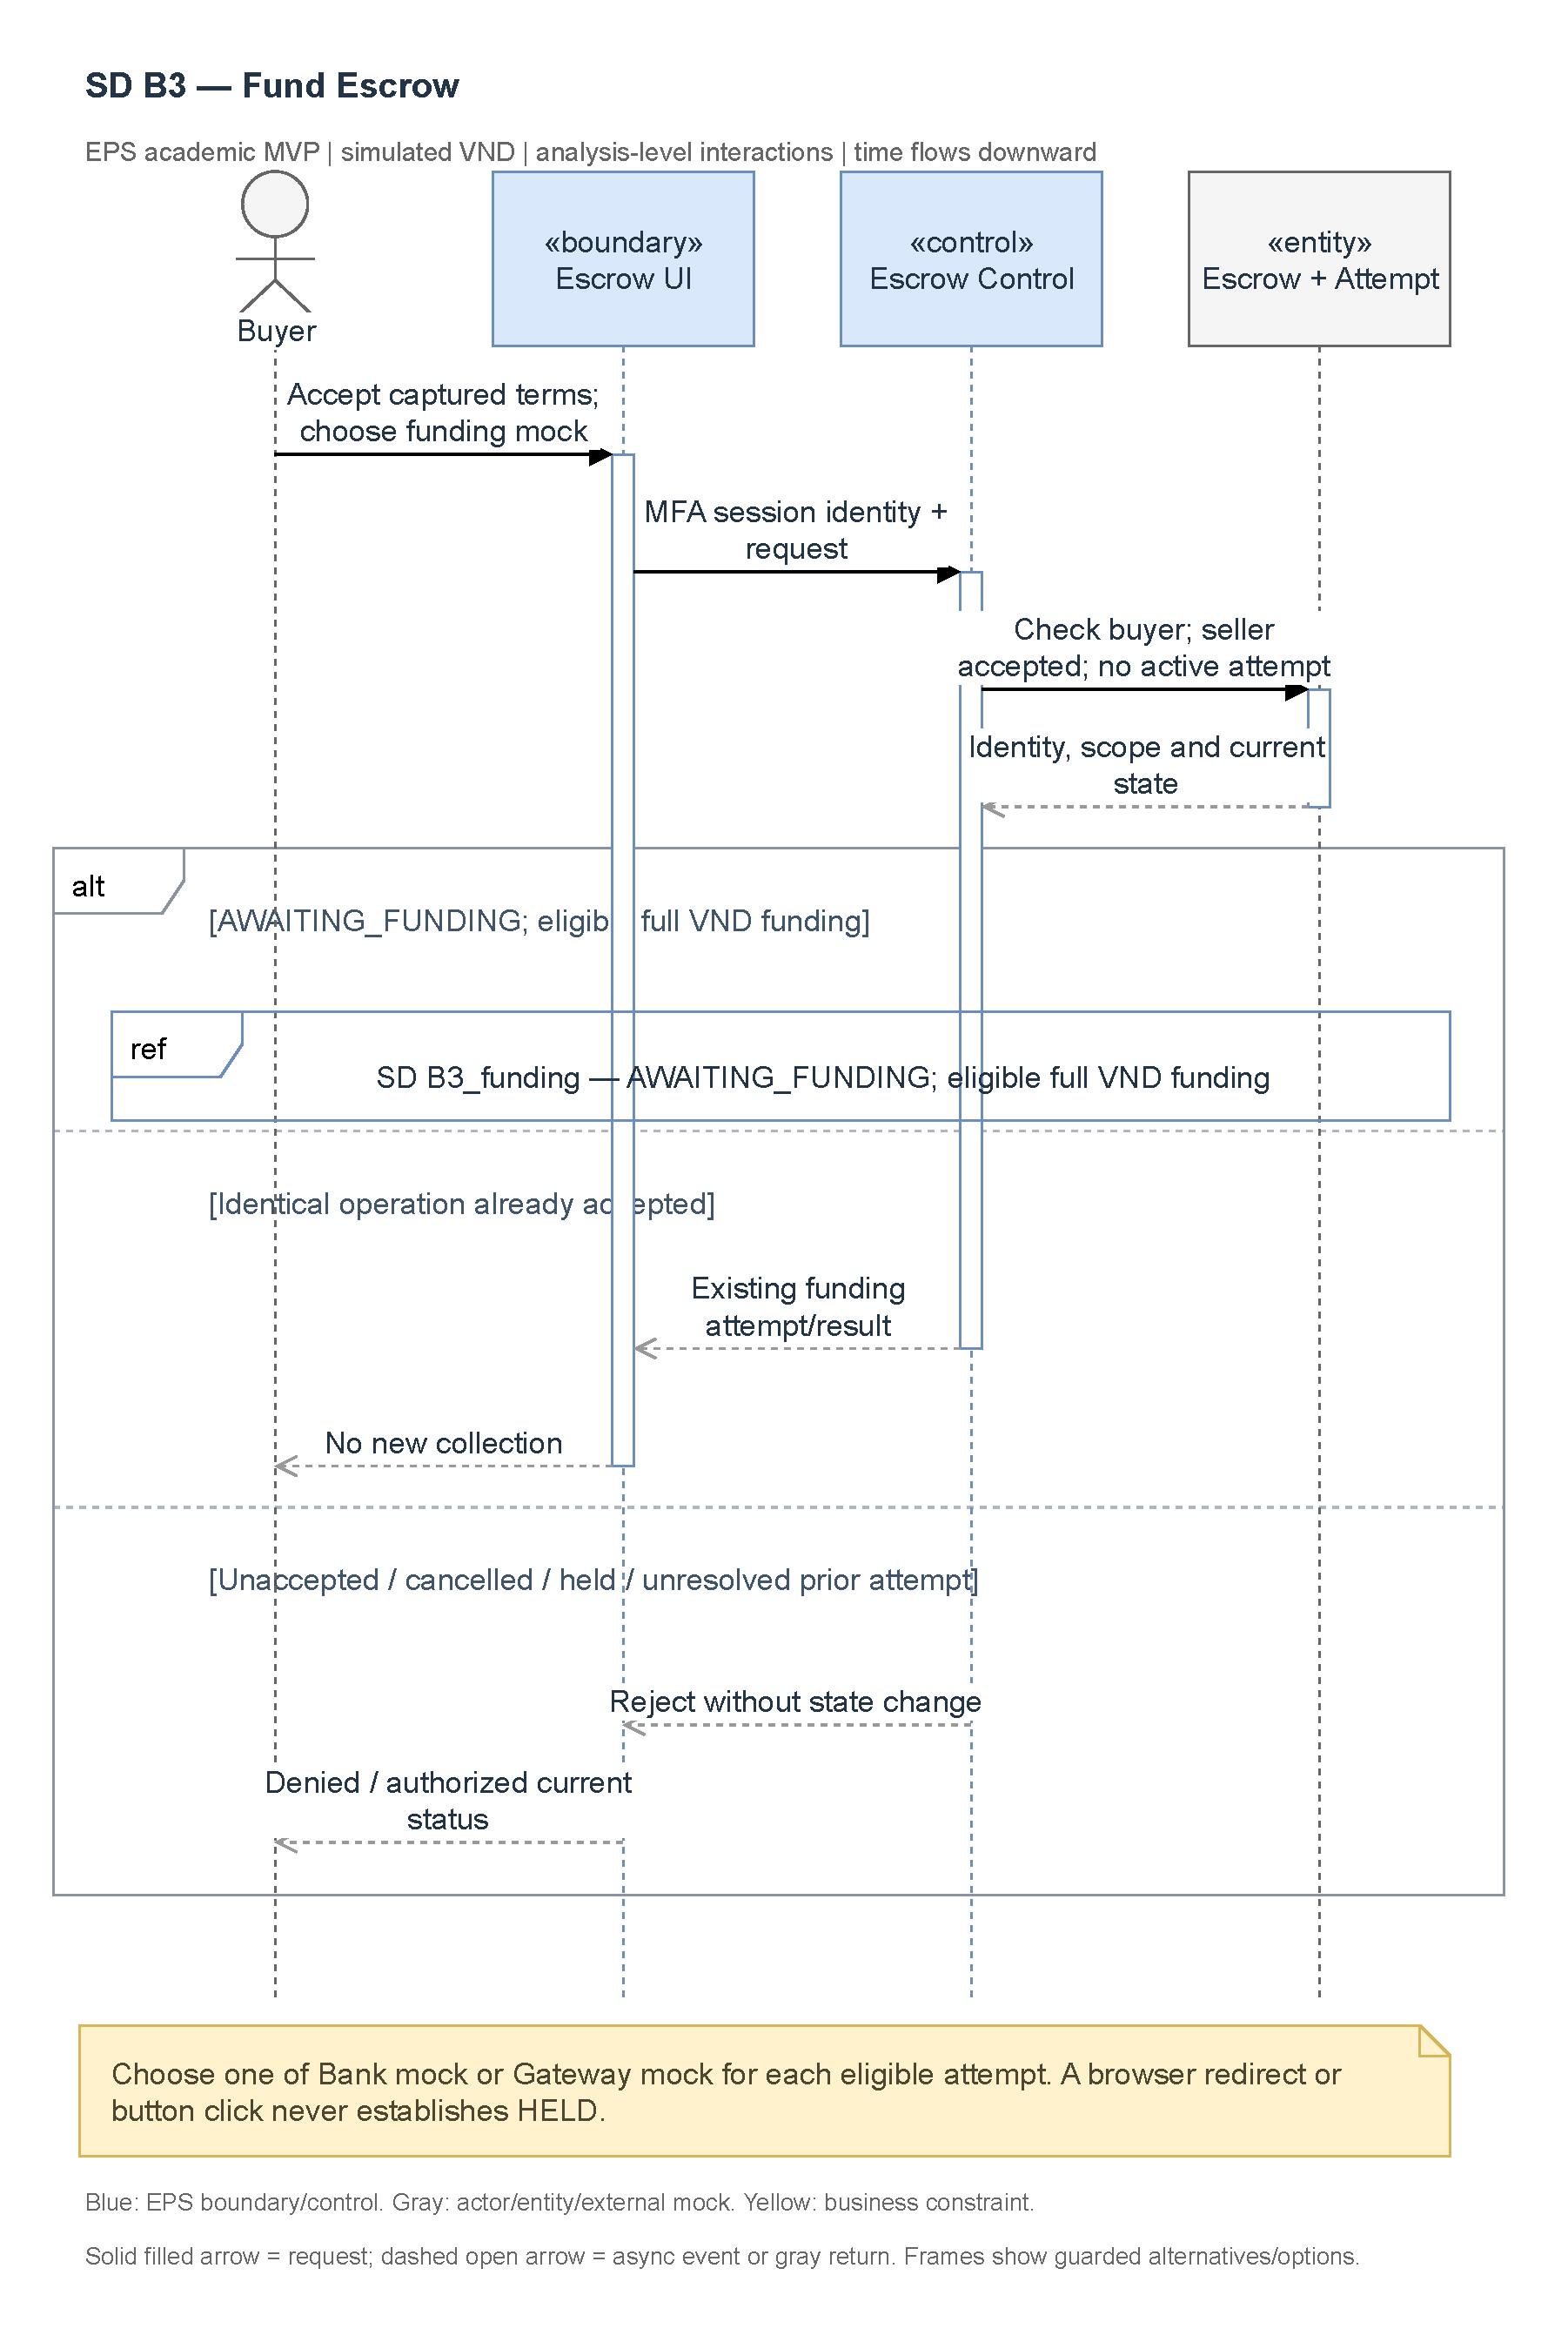
\includegraphics[width=510bp,height=700bp,keepaspectratio,clip]{diagrams/sequence/SD_B3.pdf}\caption{B3: Fund Escrow}\label{fig:sequence-b3}\end{figure}\clearpage\restoregeometry
\epsfigure{diagrams/sequence/SD_B3_funding.pdf}{B3: Fund Escrow (continued: B3\_\allowbreak{}funding)}{fig:sequence-b3-funding}
\epsfigure{diagrams/sequence/SD_B4.pdf}{B4: Confirm Acceptance and Request Release}{fig:sequence-b4}
\epsfigure{diagrams/sequence/SD_B4_outcomes.pdf}{B4: Confirm Acceptance and Request Release (continued: B4\_\allowbreak{}outcomes)}{fig:sequence-b4-outcomes}
\subsection{Seller's Use cases}
\epsfirstfigure{diagrams/sequence/SD_S1.pdf}{S1: Accept/Reject Escrow Terms}{fig:sequence-s1}
\epsfigure{diagrams/sequence/SD_S1_outcomes.pdf}{S1: Accept/Reject Escrow Terms (continued: S1\_\allowbreak{}outcomes)}{fig:sequence-s1-outcomes}
\epsfigure{diagrams/sequence/SD_S2.pdf}{S2: Record Delivery/Service Completion}{fig:sequence-s2}
\epsfigure{diagrams/sequence/SD_S2_outcomes.pdf}{S2: Record Delivery/Service Completion (continued: S2\_\allowbreak{}outcomes)}{fig:sequence-s2-outcomes}
\subsection{Admin's Use cases}
\epsfirstfigure{diagrams/sequence/SD_A1.pdf}{A1: Review and Resolve Dispute}{fig:sequence-a1}
\epsfigure{diagrams/sequence/SD_A1_decision.pdf}{A1: Review and Resolve Dispute (continued: A1\_\allowbreak{}decision)}{fig:sequence-a1-decision}
\epsfigure{diagrams/sequence/SD_A1_outcomes.pdf}{A1: Review and Resolve Dispute (continued: A1\_\allowbreak{}outcomes)}{fig:sequence-a1-outcomes}
\epsfigure{diagrams/sequence/SD_A2.pdf}{A2: Configure Escrow Policy Parameters}{fig:sequence-a2}
\epsfigure{diagrams/sequence/SD_A2_outcomes.pdf}{A2: Configure Escrow Policy Parameters (continued: A2\_\allowbreak{}outcomes)}{fig:sequence-a2-outcomes}
\epsfigure{diagrams/sequence/SD_A3.pdf}{A3: View Basic Analytics}{fig:sequence-a3}
\epsfigure{diagrams/sequence/SD_A3_outcomes.pdf}{A3: View Basic Analytics (continued: A3\_\allowbreak{}outcomes)}{fig:sequence-a3-outcomes}
\epsfigure{diagrams/sequence/SD_A4.pdf}{A4: View Audit Trail}{fig:sequence-a4}
\epsfigure{diagrams/sequence/SD_A4_outcomes.pdf}{A4: View Audit Trail (continued: A4\_\allowbreak{}outcomes)}{fig:sequence-a4-outcomes}
\epsfigure{diagrams/sequence/SD_A5.pdf}{A5: Reconcile Pending Transactions/Retry Confirmed-Failed Transfers}{fig:sequence-a5}
\epsfigure{diagrams/sequence/SD_A5_reconciliation.pdf}{A5: Reconcile Pending Transactions/Retry Confirmed-Failed Transfers (continued: A5\_\allowbreak{}reconciliation)}{fig:sequence-a5-reconciliation}
\epsfigure{diagrams/sequence/SD_A5_outcomes.pdf}{A5: Reconcile Pending Transactions/Retry Confirmed-Failed Transfers (continued: A5\_\allowbreak{}outcomes)}{fig:sequence-a5-outcomes}
\epsfigure{diagrams/sequence/SD_A5_retry.pdf}{A5: Reconcile Pending Transactions/Retry Confirmed-Failed Transfers (continued: A5\_\allowbreak{}retry)}{fig:sequence-a5-retry}
\subsection{Payment Integration's Use cases}
\epsfirstfigure{diagrams/sequence/SD_P1.pdf}{P1: Confirm Funding}{fig:sequence-p1}
\epsfigure{diagrams/sequence/SD_P1_outcomes.pdf}{P1: Confirm Funding (continued: P1\_\allowbreak{}outcomes)}{fig:sequence-p1-outcomes}
\epsfigure{diagrams/sequence/SD_P1_confirmed_receipt.pdf}{P1: Confirm Funding (continued: P1\_\allowbreak{}confirmed\_\allowbreak{}receipt)}{fig:sequence-p1-confirmed-receipt}
\epsfigure{diagrams/sequence/SD_P2.pdf}{P2: Execute and Confirm Release}{fig:sequence-p2}
\epsfigure{diagrams/sequence/SD_P2_settlement.pdf}{P2: Execute and Confirm Release (continued: P2\_\allowbreak{}settlement)}{fig:sequence-p2-settlement}
\epsfigure{diagrams/sequence/SD_P2_outcomes.pdf}{P2: Execute and Confirm Release (continued: P2\_\allowbreak{}outcomes)}{fig:sequence-p2-outcomes}
\epsfigure{diagrams/sequence/SD_P3.pdf}{P3: Execute and Confirm Refund}{fig:sequence-p3}
\epsfigure{diagrams/sequence/SD_P3_settlement.pdf}{P3: Execute and Confirm Refund (continued: P3\_\allowbreak{}settlement)}{fig:sequence-p3-settlement}
\epsfigure{diagrams/sequence/SD_P3_outcomes.pdf}{P3: Execute and Confirm Refund (continued: P3\_\allowbreak{}outcomes)}{fig:sequence-p3-outcomes}

\end{document}
